\documentclass[a4paper,12pt]{article}

\usepackage{graphicx} % Required for inserting images
\usepackage{amsmath,amssymb,amsfonts}
\usepackage{subcaption}
% -----------------------
% Package Imports
% -----------------------

% Set page margins
\usepackage[a4paper, top=1in, bottom=0.8in, left=1.1in, right=0.8in]{geometry}

% Use Times New Roman font
\usepackage{times}
\usepackage{pdfpages} % Include PDF files





% Set page margins
\usepackage[a4paper, top=1in, bottom=0.8in, left=1.1in, right=0.8in]{geometry}


% Add page numbering
\pagestyle{plain}

% Enable graphics inclusion
\usepackage{graphicx}
\usepackage{float}
% Enable code listings
\usepackage{listings}
\usepackage{xcolor} % For customizing code colors
\setlength{\parindent}{0pt}
\usepackage{multirow}

\setlength{\parindent}{0pt}
\usepackage{titlesec} % To customize section font size
\titleformat{\section}
{\normalfont\fontsize{14}{16}\bfseries}{\thesection}{1em}{}

\titleformat{\subsection}
{\normalfont\fontsize{14}{16}\bfseries}{\thesubsection}{1em}{}

\begin{document}
	\section{Experiment No. 6}
	
	\section{Experiment Title }
	Determination of V-Curve of a synchronous motor.
	
	\section{Objective}
	
	The objectives of this lab are as follows:
	\begin{itemize}
		\item 	To study the variation of armature current with respect to the field current in a synchronous motor under constant load
		\item 	To determine the V-Curve of a synchronous motor by plotting a graph of field current versus armature current.
		
		\item 	To understand the over-excited and under-excited operating conditions of a synchronous motor.
		
		
	\end{itemize}
	
	\section{Theory}
	
	A synchronous motor operates at a constant speed synchronized with the frequency of the supply voltage. One of its distinguishing features is the ability to control its power factor by varying the excitation (field) current. The rotor winding is excited with direct current (DC) through slip rings, while the stator is powered by a three-phase alternating current (AC) supply.
	
	Depending on the excitation level, the motor operates in the following modes:
	\begin{itemize}
		\item \textbf{Under-Excited:} The motor draws a lagging current, similar to an inductive load.
		\item \textbf{Normal-Excited:} The motor operates at unity power factor.
		\item \textbf{Over-Excited:} The motor draws a leading current, like a capacitive load.
	\end{itemize}
	
	\subsection*{V-Curve of Synchronous Motor}
	The V-curve is a plot of armature current ($I_A$) versus field current ($I_f$) at constant mechanical load. The curve resembles the shape of the letter "V". As the field current increases:
	\begin{itemize}
		\item The armature current initially decreases.
		\item At unity power factor, $I_A$ is minimum.
		\item Beyond this point, $I_A$ increases again with over-excitation.
	\end{itemize}
	
	This behavior is due to the interplay between excitation and the motor’s reactive power behavior.
	
	\subsection*{Voltage Equation of a Synchronous Motor}
	
	The synchronous motor voltage equation is given by:
	
	\begin{equation}
		E_A = V_\phi - I_A R_A - jX_s I_A
	\end{equation}
	
	Where:
	\begin{itemize}
		\item $E_A$ = Internal generated voltage (back EMF)
		\item $V_\phi$ = Terminal phase voltage
		\item $I_A$ = Armature current
		\item $R_A$ = Armature resistance
		\item $X_s$ = Synchronous reactance
	\end{itemize}
	
	\subsection*{Power Developed by the Motor}
	
	The real power developed by a synchronous motor is:
	
	\begin{equation}
		P = \frac{E_A V_\phi}{X_s} \sin \delta
	\end{equation}
	
	Where:
	\begin{itemize}
		\item $P$ = Power output
		\item $\delta$ = Torque angle (also called power angle)
	\end{itemize}
	
	For a \textbf{generator}, $\delta$ is positive, indicating power supply. For a \textbf{motor}, $\delta$ is negative, signifying power consumption.
	
	\subsection*{Types of Synchronous Motors}
	Synchronous motors can be classified into two major types:
	\begin{enumerate}
		\item \textbf{Non-Excited Synchronous Motors}
		\item \textbf{Direct Current (DC) Excited Synchronous Motors}
	\end{enumerate}
	
	Excited synchronous motors can be further categorized as:
	\begin{itemize}
		\item \textbf{Under-Excited:} $V_\phi$ lags $E_A$
		\item \textbf{Over-Excited:} $V_\phi$ leads $E_A$
	\end{itemize}
	
	\subsection*{Armature Current Behavior with Field Current}
	As the excitation voltage ($E_A$) increases, the armature current ($I_A$) initially decreases, reaching a minimum at unity power factor. This is followed by an increase in $I_A$ as $E_A$ continues to increase. The armature current behavior is as follows:
	\begin{itemize}
		\item At low $E_A$, $I_A$ lags and the motor consumes reactive power.
		\item At unity power factor, $I_A$ aligns with $V_\phi$ and behaves as a resistive load.
		\item At high $E_A$, $I_A$ leads and the motor supplies reactive power to the system.
	\end{itemize}
	
	\subsection*{Graphical Representation}
	Plotting the field current ($I_f$) on the x-axis and the armature current ($I_A$) on the y-axis results in a characteristic “V” shape, known as the V-curve of a synchronous motor.
	
	% Insert figure placeholder
	% \begin{figure}[H]
		%     \centering
		%     \includegraphics[width=0.5\textwidth]{vcurve.png}
		%     \caption{V-Curve: Variation of Armature Current ($I_A$) with Field Current ($I_f$)}
		% \end{figure}
	


	\section{Circuit Diagram}
	\begin{figure}[H]
		\centering
		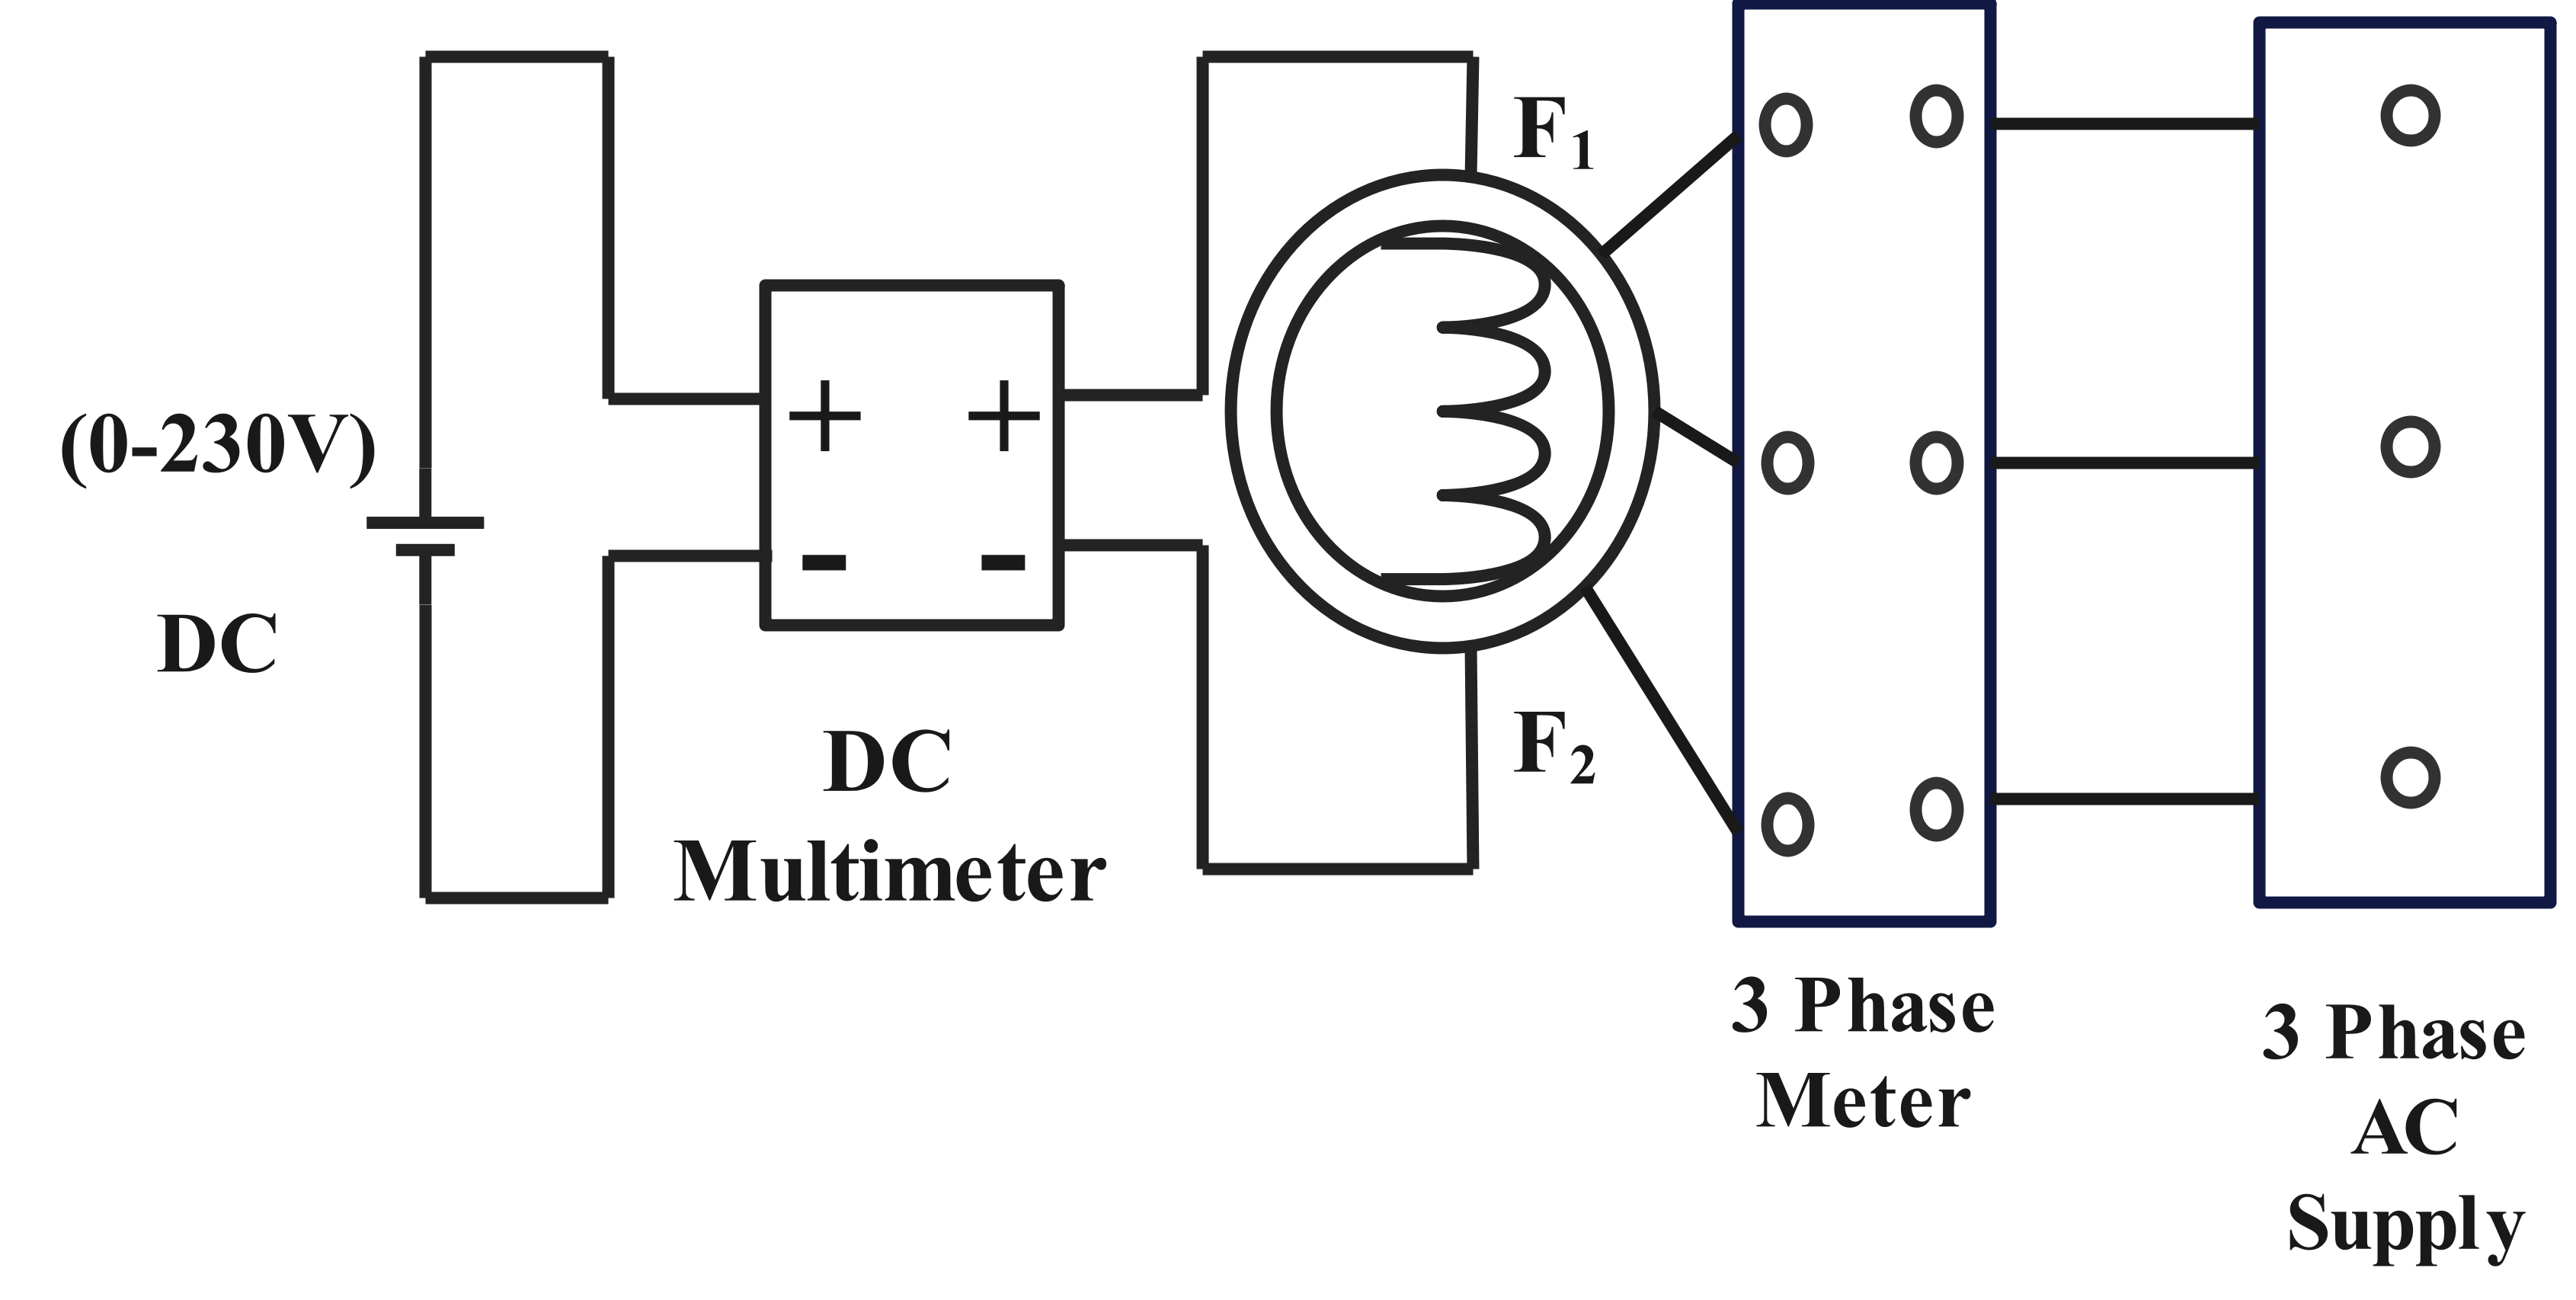
\includegraphics[width=0.7\textwidth]{Images/3}
		\caption{Experimental setup for obtaining V curve}
		
	\end{figure}
	
	
	
	\section{Required Apparatus}
	
	\begin{enumerate}
		\item Three-phase synchronous motor [Rated: \(U = 400\,\text{V (Y)} / 230\,\text{V}(\Delta),\ I = 0.57\,\text{A}/1\,\text{A},\ I_\text{exc} = 0.45\,\text{A}\)]
		\item Variable DC source [Rated: \(0\text{–}230\,\text{V},\ 3\,\text{A}\)]
		\item Tachogenerator [Rated: \(I = 0.07\,\text{A max},\ n = 5000\,\text{rpm max}\)]
		\item DC multimeter [Rated: \(600\,\text{V} – 20\,\text{A}\)]
		\item AC multimeter [Rated: \(500\,\text{V rms max},\ 5\,\text{A max}\)]
		\item Connecting wires
		\item 3-phase fixed AC supply
	\end{enumerate}
	

	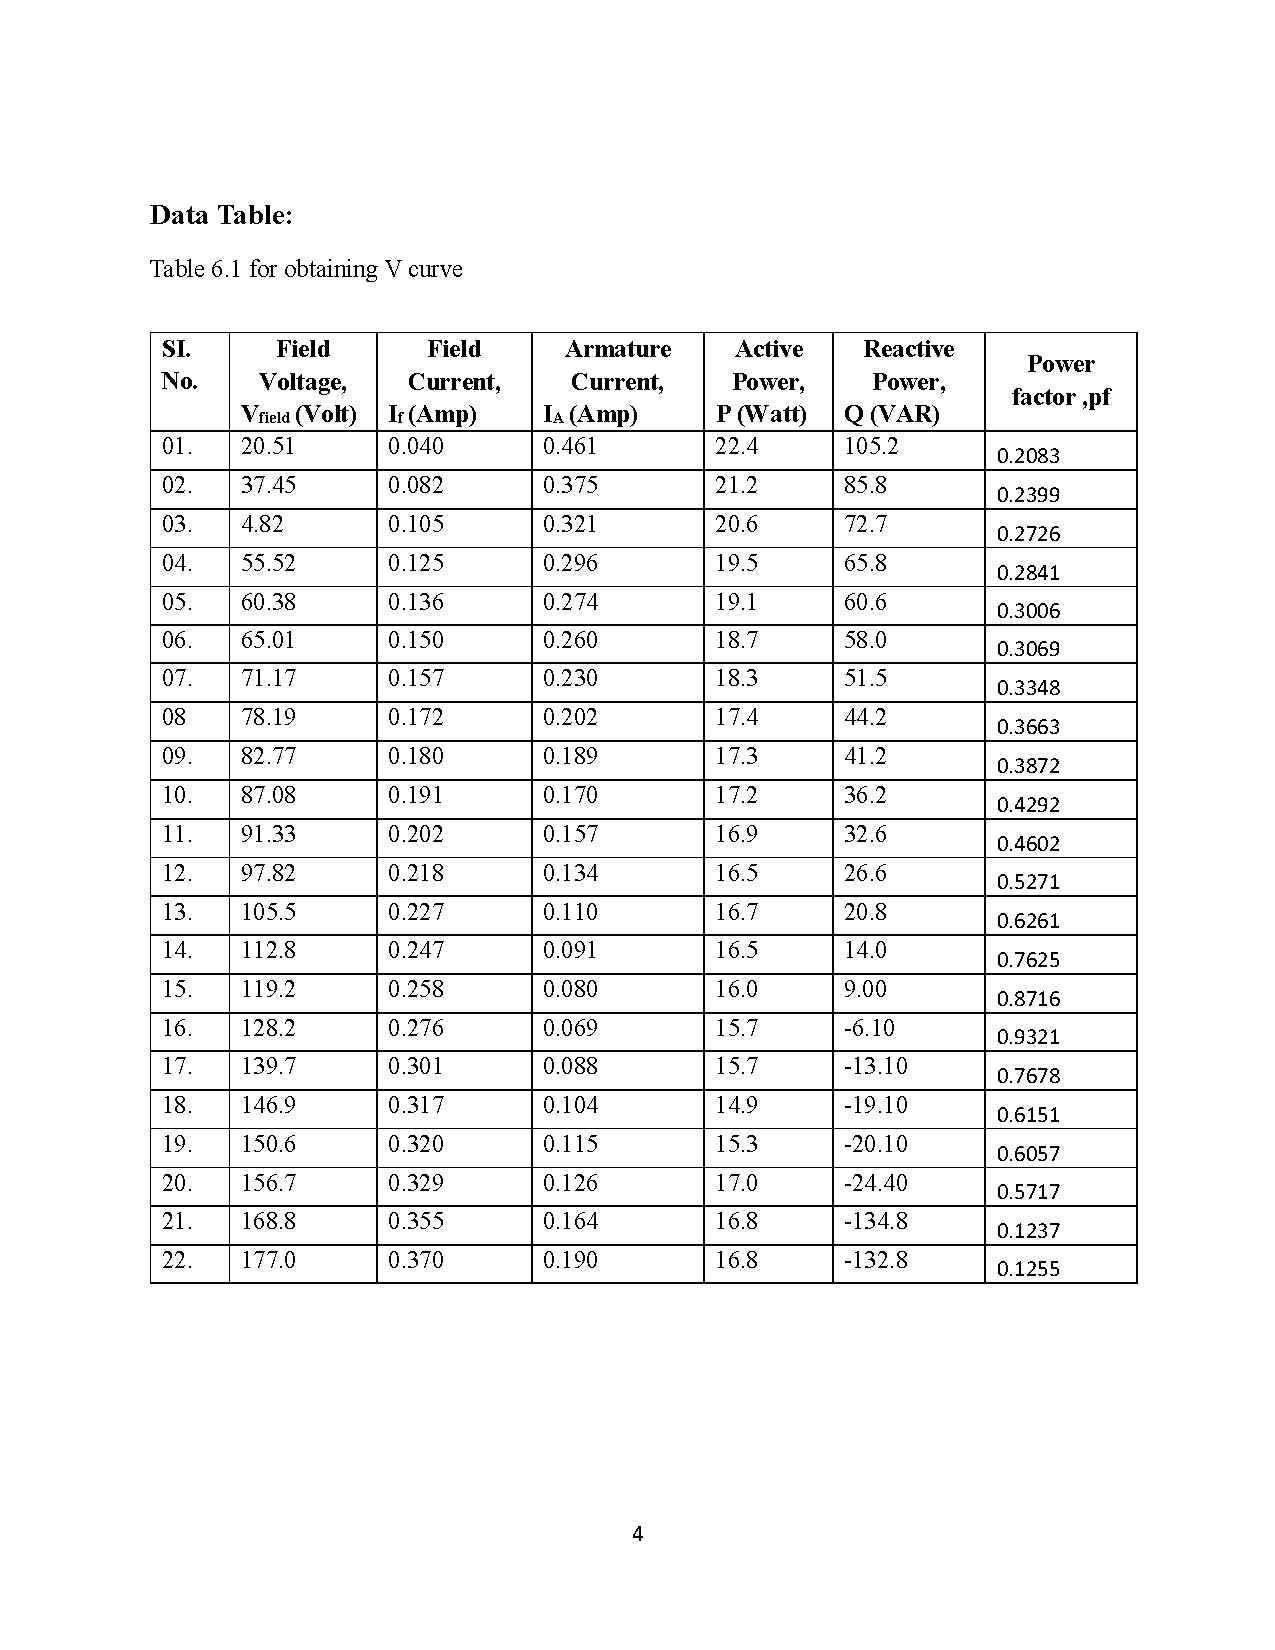
\includepdf[pages=-, fitpaper=true]{datatable.pdf}

\section{Graph}
	\begin{figure}[H]
	\centering
	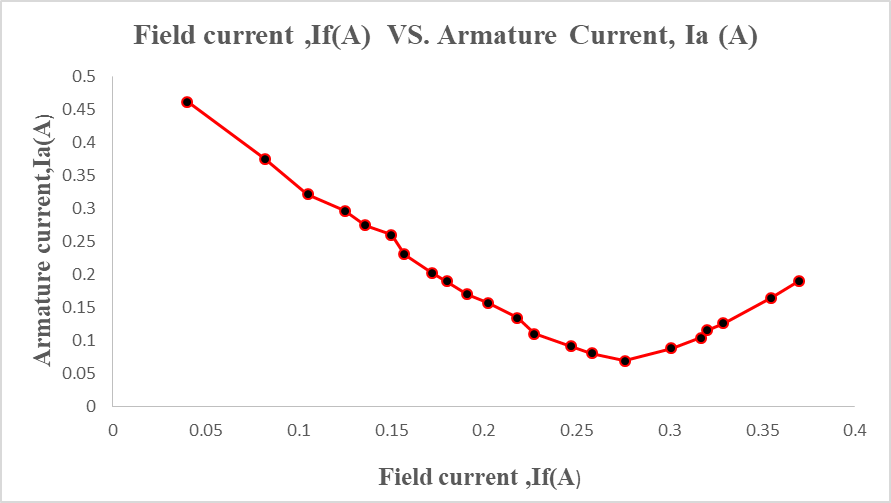
\includegraphics[width=0.79\linewidth]{Images/2}
	\caption{Obtained V curve of a synchronous motor}
	\label{fig:1}
\end{figure}
\begin{figure}[H]
	\centering
	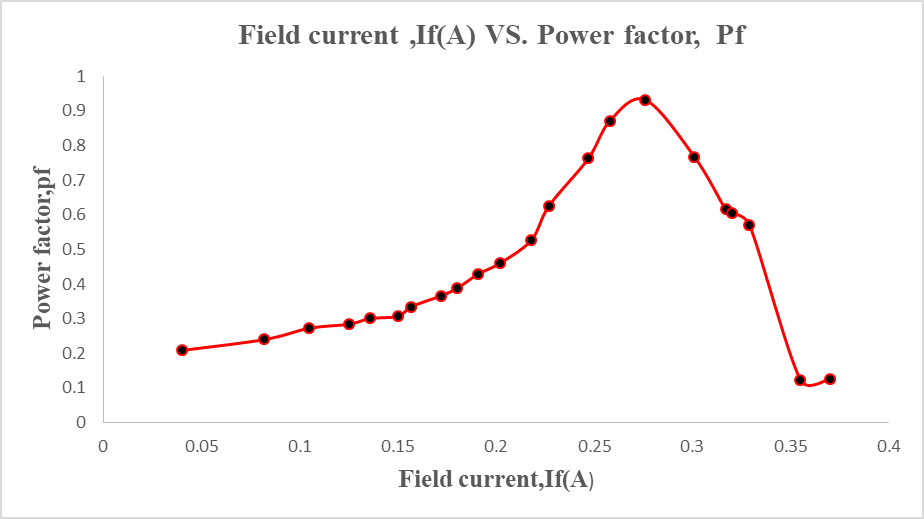
\includegraphics[width=0.79 \linewidth]{Images/1}
	\caption{Obtained V curve of a synchronous motor}
	\label{fig:2}
\end{figure}

	
	\section{Discussion}
	


In this experiment, the effect of field current on the armature current and power factor of a synchronous motor was observed. It was found that the armature current decreased to a minimum at normal excitation, corresponding to a unity power factor, and then increased with further excitation. From the V-curve, it was evident that under-excitation resulted in a lagging power factor, while over-excitation led to a leading power factor, as shown in the inverse V-curve. These results demonstrated that the power factor of a synchronous motor could be effectively controlled by adjusting the excitation level.

	
	
	Overall, the experiment effectively demonstrated the critical role of the auxiliary winding and capacitor in enabling self-starting in single-phase induction motors.
	
	
	
	
\end{document}
